\documentclass{article}
\setlength{\parskip}{5pt} % esp. entre parrafos
\setlength{\parindent}{0pt} % esp. al inicio de un parrafo
\usepackage{amsmath} % mates
\usepackage[sort&compress,numbers]{natbib} % referencias
\usepackage{url} % que las URLs se vean lindos
\usepackage[top=25mm,left=20mm,right=20mm,bottom=25mm]{geometry} % margenes
\usepackage{hyperref} % ligas de URLs
\usepackage{graphicx} % poner figuras
\usepackage[spanish]{babel} % otros idiomas
\usepackage[utf8]{inputenc}
\author{Karla Ocañas \\ Gabryiel Bailon \\ Miguel Rodrigo \\ Alfredo Llanes \\ Betsaida Ruedas} % author
\title{Tarea 1} % titulo
\date{\today}

\begin{document} % inicia contenido

\maketitle % cabecera

\begin{abstract} % resumen
Su objetivo es identificar alteraciones o desajustes que se producen durante el movimiento para así proponer métodos de intervención que mejoren el desempeño, la salud y calidad de vida del paciente.\\
\\
Gracias a los avances de la ciencia y la tecnología durante los últimos años, las posibilidades que ofrece la Biomecánica aplicada al deporte han ido creciendo, todas ellas con un mismo factor común, mejorar el rendimiento del deportista y reducir el riesgo de sufrir lesiones mediante el análisis y corrección del movimiento.
\\
\\
Hoy en día cualquier persona que practica deporte, independientemente de su nivel, corre el riesgo de sufrir dolores o lesiones al realizar un movimiento o gesto de manera incorrecta repetidas veces cuando practica deporte. Este riesgo por supuesto es mayor en deportistas de alto nivel debido al elevado número de horas de entreno que realizan.\\

\end{abstract}


\section{Introducci\'{o}n}\label{intro} % seccion y etiqueta
El fin que tiene la actividad de este documento es poder tener los conocimientos para introducirnos a la biomecanica, es decir, poder adentrarnos en los conceptos mas basicos de la ingenieria en la mecanica, sobre biologica, anatomia, etc para poder abordar temas mas complejos como la contruccion de protesis humanas, desarrollo de ideas biotecnologicas etcetera.  


\section{Desarrollo}

\cite{ff1}\textbf{¿Qué es la biomecanica?} \\
\\
La biomecánica es la ciencia que estudia el movimiento y actividades de los seres vivos en diferentes situaciones, junto a la componente mecánica y la energía incluidas en ellas, es decir, la relación que existe entre fuerza y movimiento en los seres vivos. \\
\textbf Este ámbito se trata de un área interdisciplinaria, que se centra tanto en el cuerpo humano como en otros organismos.
A la hora de querer entender qué es la biomecánica humana, ha de tenerse en cuenta que esta disciplina estudia las fuerzas internas y externas ejercidas sobre el cuerpo humano, para analizar los efectos producidos. Por tanto, en biomecánica, esta definición puede ser igualmente válida en cuanto a ciencia que estudia el cuerpo humano.
la biomecánica emplea los conocimientos de la mecánica, la anatomía, la fisiología, ingeniería, y de otras disciplinas en las cuales se apoya para llegar a entender el efecto producido en nuestro cuerpo.\\
\\
\textbf {Ramas de la Biomecánica} \\

\begin{description}
\item •	Biomecánica médica: Analiza patologías que afectan al hombre y la mujer, (biomecánica humana), con el fin de evaluar, paliar o reparar los daños
\item •	Biomecánica ocupacional: Aplicando la biomecánica del cuerpo humano, adapta a este sus necesidades y capacidades estudiando su interacción con aquellos elementos con los cuales se relaciona en distintos ámbitos, ya sea en casa, en el automóvil, manejando herramientas o en el trabajo, (biomecánica laboral), entre otros contextos.
\item •	Biomecánica fisioterapéutica: Realiza una evaluación de las disfunciones del sistema musculo esquelético, en seres humanos, para observarlas, tratarlas y reducirlas.
\item •	Biomecánica deportiva: Desarrolla técnicas de entrenamiento y diseña complementos, equipamientos y materiales de altas prestaciones, mediante el análisis de la práctica deportiva, para favorecer la biomecánica del movimiento. 
\item •	Biomecánica forense: Indaga en ciencia que estudia el movimiento para analizar cada mecanismo de lesión, producido por el cuerpo, ante accidentes, colisiones, choques u otro tipo de acciones de esfuerzo considerables
\end{description}

\begin{figure} [htp]% figura
    \centering
    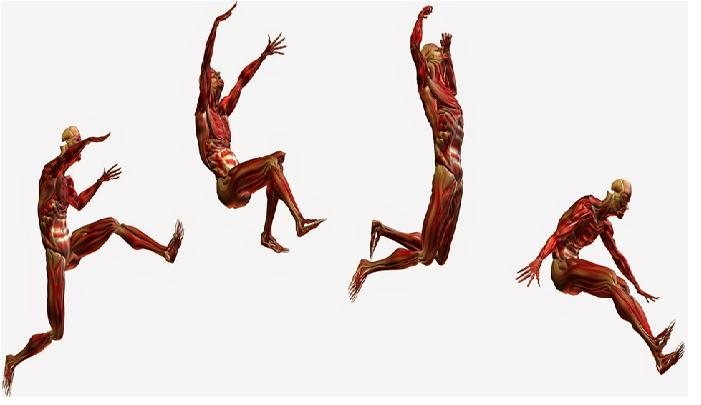
\includegraphics[width=150mm]{biomecanica1.jpg} % archivo
    \caption{Musculos del cuerpo en movimiento}
    \label{grafica}
\end{figure}


\textbf{¿Que es la mecanica?} \\
La mecánica es la parte de la Física que estudia el movimiento de los cuerpos como consecuencia de las fuerzas que actúan sobre ellos.
Se divide en dos partes: \\
 \\

\begin{description}
\item •	Cinemática: Describe el movimiento de los cuerpos sin tener en cuenta las causas que lo producen.
\item •	Dinámica: Estudia la relación entre las fuerzas que actúan sobre un cuerpo y los efectos que producen.

\item Estática, comprendida dentro de la dinámica, analiza las condiciones que producen el equilibrio de los cuerpos, como consecuencia de las fuerzas que actúan sobre ellos.\\
\\
La aplicación de los principios de la mecánica al estudio del cuerpo humano y de los seres vivos se conoce como biomecánica.\\
\\
\end{description} 

\begin{figure} [htp]% figura
    \centering
    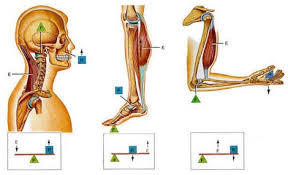
\includegraphics[width=150mm]{biomecanica2.jpg} % archivo
    \caption{Representación de la mecanica en la Biomecánica}
    \label{grafica}
\end{figure}

\cite{ff2}\textbf{Anatomia de la mano} \\

\begin{description}
\item •	Huesos de la mano:El esqueleto de los dedos está formado por pequeños huesos largos llamados falanges en número de tres para cada dedo menos el primer dedo que solo tiene dos, carece de la central.\\ La palma de la mano está constituida por cinco huesos largos llamados metacarpianos que se articulan distalmente con las primeras falanges de los dedos y próximamente con ocho huesos que constituyen las dos filas del carpo que vistas en posición anatómica serian en la primera fila de proximal a distal el hueso escafoides, semilunar, piramidal y pisiforme, la fila distal seria trapecio, trapezoide grande y ganchoso.\\

\begin{figure} [htp]% figura
    \centering
    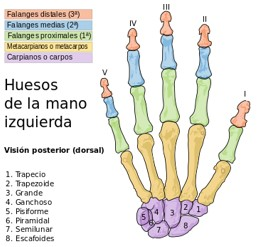
\includegraphics[width=70mm]{biomecanica3.jpg} % archivo
    \caption{Huesos de la mano}
    \label{grafica}
\end{figure}

\item •Articulaciones de la mano:  Los huesos de la mano se articulan entre sí de forma diferente obedeciendo al principio de la funcionabilidad morfológica, es decir cada hueso presenta superficies articulares cubiertas de cartílago que permite la contigüidad de los huesos para mantener la armazón interna de la mano, pero que a la vez están dotados de elementos blandos pasivos y activos que permiten que en la coyuntura se produzca o no el desplazamiento de los segmentos óseos articulares.\\ Al nivel de las articulaciones metacarpofalángicas se produce una articulación elipsoide que por tanto se comporta igual que la radiocarpiana con los mismos ejes y movimientos.\\

\begin{figure} [htp]% figura
    \centering
    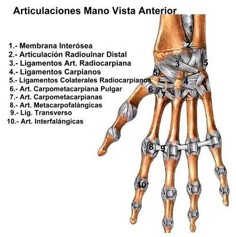
\includegraphics[width=70mm]{biomecanica4.jpg} % archivo
    \caption{Articulaciones de la mano}
    \label{grafica}
\end{figure}

\item •Músculos Intrínsecos : Se distribuyen en pequeños grupos en la mano por la cara palmar en la porción cubital encontramos la eminencia hipotenar donde vamos a encontrar pequeños músculos vinculados todos con los movimientos del quinto dedo y que su acción al igual que los demás se precisa por su nombre.\\ De ellos señalaremos topográficamente el palmar cutáneo, el flexor corto el abductor y el oponente del quinto dedo.\\

\begin{figure} [htp]% figura
    \centering
    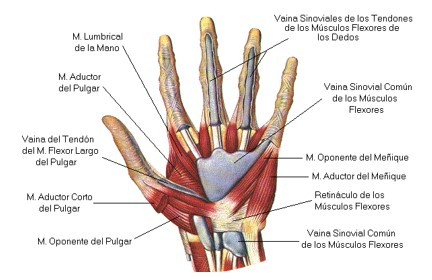
\includegraphics[width=100mm]{biomecanica5.jpg} % archivo
    \caption{musculos de la mano}
    \label{grafica}
\end{figure}


\item •Músculos Extrínsecos : Son los encargados de los movimientos de gran amplitud y potencia de los dedos se encuentran situados en el antebrazo en su tercio superior.\\ Es importante destacar que todos estos músculos incluyendo los no situados en la mano sino en el antebrazo son los que garantizan la motilidad de la mano.\\
\end{description}

\\

\section{Conclusiones}

La biomecánica, a diferencia de los exámenes de diagnóstico por la imagen, que se utilizan habitualmente, y que son pruebas estáticas, de tipo morfológico, (como la resonancia magnética, el escáner y la radiografía), permite la realización de mediciones precisas de los movimientos, según resalta la doctora Ulldemolins, siendo una prueba complementaria más.\\
\\
”Muchas enfermedades pueden ser muy bien evaluadas desde el punto de vista anatómico, pero, sin embargo, en algunos casos la interpretación originada en estudios estáticos no permite una clara evaluación de la disfunción derivada de las patologías osteoarticulares”, añade.\\
\\
A su vez, resalta que las pruebas biomecánicas se han venido utilizando básicamente para valorar las limitaciones funcionales reales de trabajadores para las mutuas laborales o como pruebas periciales en casos judiciales o en accidentes de tráfico, pero “cada vez más”, y gracias a la investigación y a la innovación, encontramos nuevas aplicaciones de la biomecánica en los procesos de rehabilitación tras una lesión, una intervención quirúrgica, e incluso vemos que esta disciplina ayuda a reducir el tiempo de la adaptación a las prótesis de un miembro amputado.
\\

\bibliography{bib}
\bibliographystyle{plainnat}

\end{document}